\section{Definition eines Stromflusses, Octave}
Wir betrachten nun das Problem zwei parallel verlaufender Kabel (siehe Abb. \ref{fig:problem}). Kabel 1 soll den Strom $1 \si{\ampere}$ und Kabel 2 entgegengesetzt $-1\si{\ampere}$ führen. Angenommen wird, dass die magnetische Flussdichte an den Randflächen $\Gamma$ des Rechengebiets abgeklungen ist und 
\begin{equation}
\label{rand}
\vec{A}_t(\vec{r}) = 0 \qquad \text{für alle } \vec{r} \in \Gamma
\end{equation}
gilt.

\begin{figure}[thbp]
	\centering
	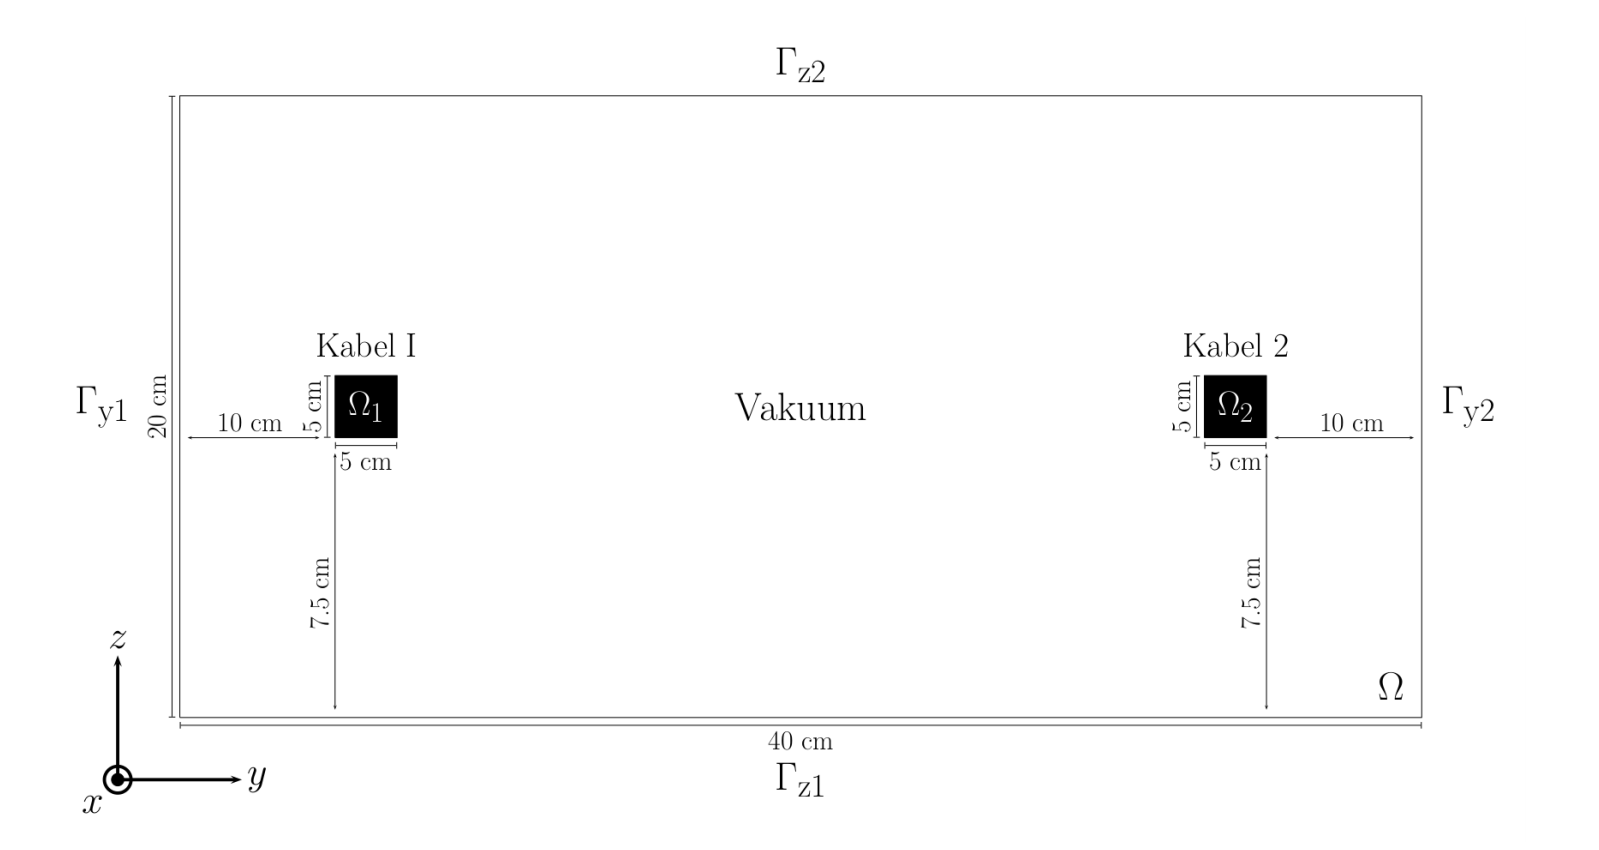
\includegraphics[width=.75\textwidth]{data/Problem}
	\caption{Zwei Kabel in der $yz$-Ebene}
	\label{fig:problem}
\end{figure}

Für die Simulation wird ein äquidistantes Rechengitter definiert. Wir haben uns dazu entschieden zu Testzwecken zunächst einmal ein sehr grobes Gitter zu wählen, mit Anzahl Knoten $N_x=2, N_y=9, N_z=9$ und einer Schrittweite $h_x=20\si{\centi\meter},h_y=5\si{\centi\meter},h_z=2,5\si{\centi\meter}$ (siehe Code (\ref{ag3})). Mithilfe der zuvor geschriebenen Methoden \texttt{fit\_operator} (\ref{fit}) wird der benötigte FIT-Operator $\mb{C}$ erzeugt. Es folgt die Bestimmung der Indexmenge \texttt{indxT} aller Randkanten, die wir als Vektor definiert haben. Hierbei werden erst alle Kanten in x-Richtung durch gegangen, daran angehängt die in y- und z-Richtung. Im Vektor steht nun entweder eine $1$, falls die Kante eine Randkante ist, ansonsten eine $0$.

Ähnlich wird bei Bestimmung des Anregungsvektors $\vec{j}$ vorgegangen. Der Vektor wird am Index einer Kante, die zum einen in $\Omega_1$ oder $\Omega_2$ liegt und zusätzlich in Stromrichtung (also x-Richtung) zeigt, auf $\pm1$ gesetzt. Anschließend wird der Vektor noch mit dem Faktor $\left(\dfrac{h_x}{5\si{\centi\meter}}\right)^2$ multipliziert.

Nun soll die Gleichung
\begin{equation}
\label{Kaj}
	\mb{K}\vec{a} = \vec{j} \qquad \text{mit } \mb{K} = \mb{C}^T\mb{M}_v\mb{C}
\end{equation}
gelöst werden. Hierzu wird zunächst noch mithilfe der schon geschriebenen Routine \texttt{createMny} (\ref{Matmatrix}) die Matrix $\mb{M}_v$ erzeugt. Das magnetische Vektorpotential $\vec{a}$ enthält momentan schon Werte die uns bekannt sind, jene, die durch die Randbedingung (\ref{rand}) festgelegt sind. Es wird eine Zerlegung des Gleichungssystems in Bekannte und Unbekannte vorgenommen. Hierzu werden aus dem Gleichungssystem (\ref{Kaj}) alle Gleichungen entfernt die Randkanten beschreiben. Mithilfe des Vektors \texttt{indxT} werden in $\mb{K}$ und $\vec{j}$ alle Zeilen (bzw. bei $\mb{K}$ auch die Spalten) gelöscht, die dem Index einer Randkante entsprechen. Das verkleinerte Gleichungssystem lässt sich nun eindeutig lösen. Die Randbedingung fungiert als eine Form von Eichung.

Zuletzt können nun noch die beiden Gleichungen
\begin{align*}
\vec{b} &= \mb{C}\vec{a},\\
L &= (\vec{j})^T \dfrac{\vec{a}}{I^2}
\end{align*}
berechnet werden (siehe Code (\ref{ag3}))

Eine Simulation in FEMM ergab das resultierende magnetische Feld (Abb. \ref{fig:magnet}) und den Stromfluss (Abb. \ref{fig:strom}). Der Stromfluss verhält sich nach dem Skineffekt so wie erwartet (Am Rand des Kabels ist ein erhöhter Stromfluss erkennbar). Wieder den Erwartungen verhält sich jedoch das Magnetfeld (Abb. \ref{fig:magnet}) durch Bedingung (\ref{rand}) sollte es am Rand des Rechengebiets $0$ sein.

\begin{figure}[thbp]
	\centering
	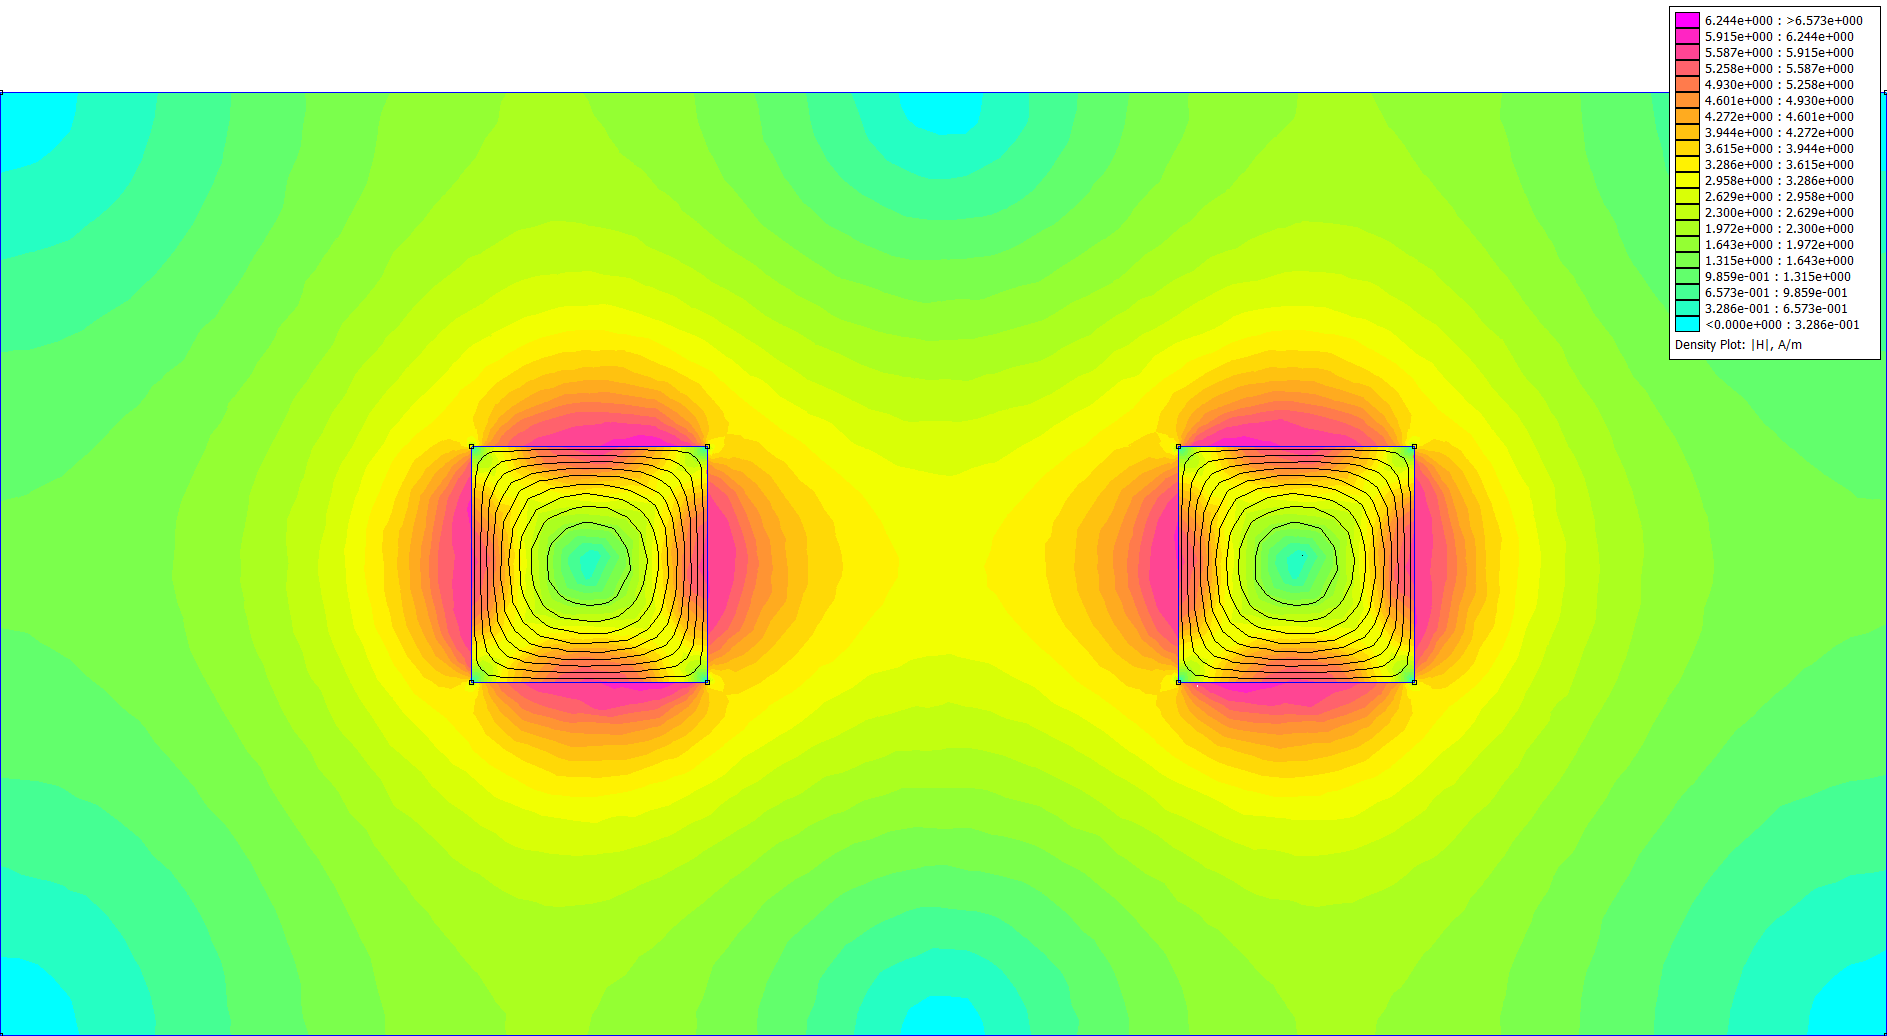
\includegraphics[width=.68\textwidth]{data/MagnetischesFeld}
	\caption{Simulation des Magnetischen Feldes in FEMM}
	\label{fig:magnet}
\end{figure}

\begin{figure}[thbp]
	\centering
	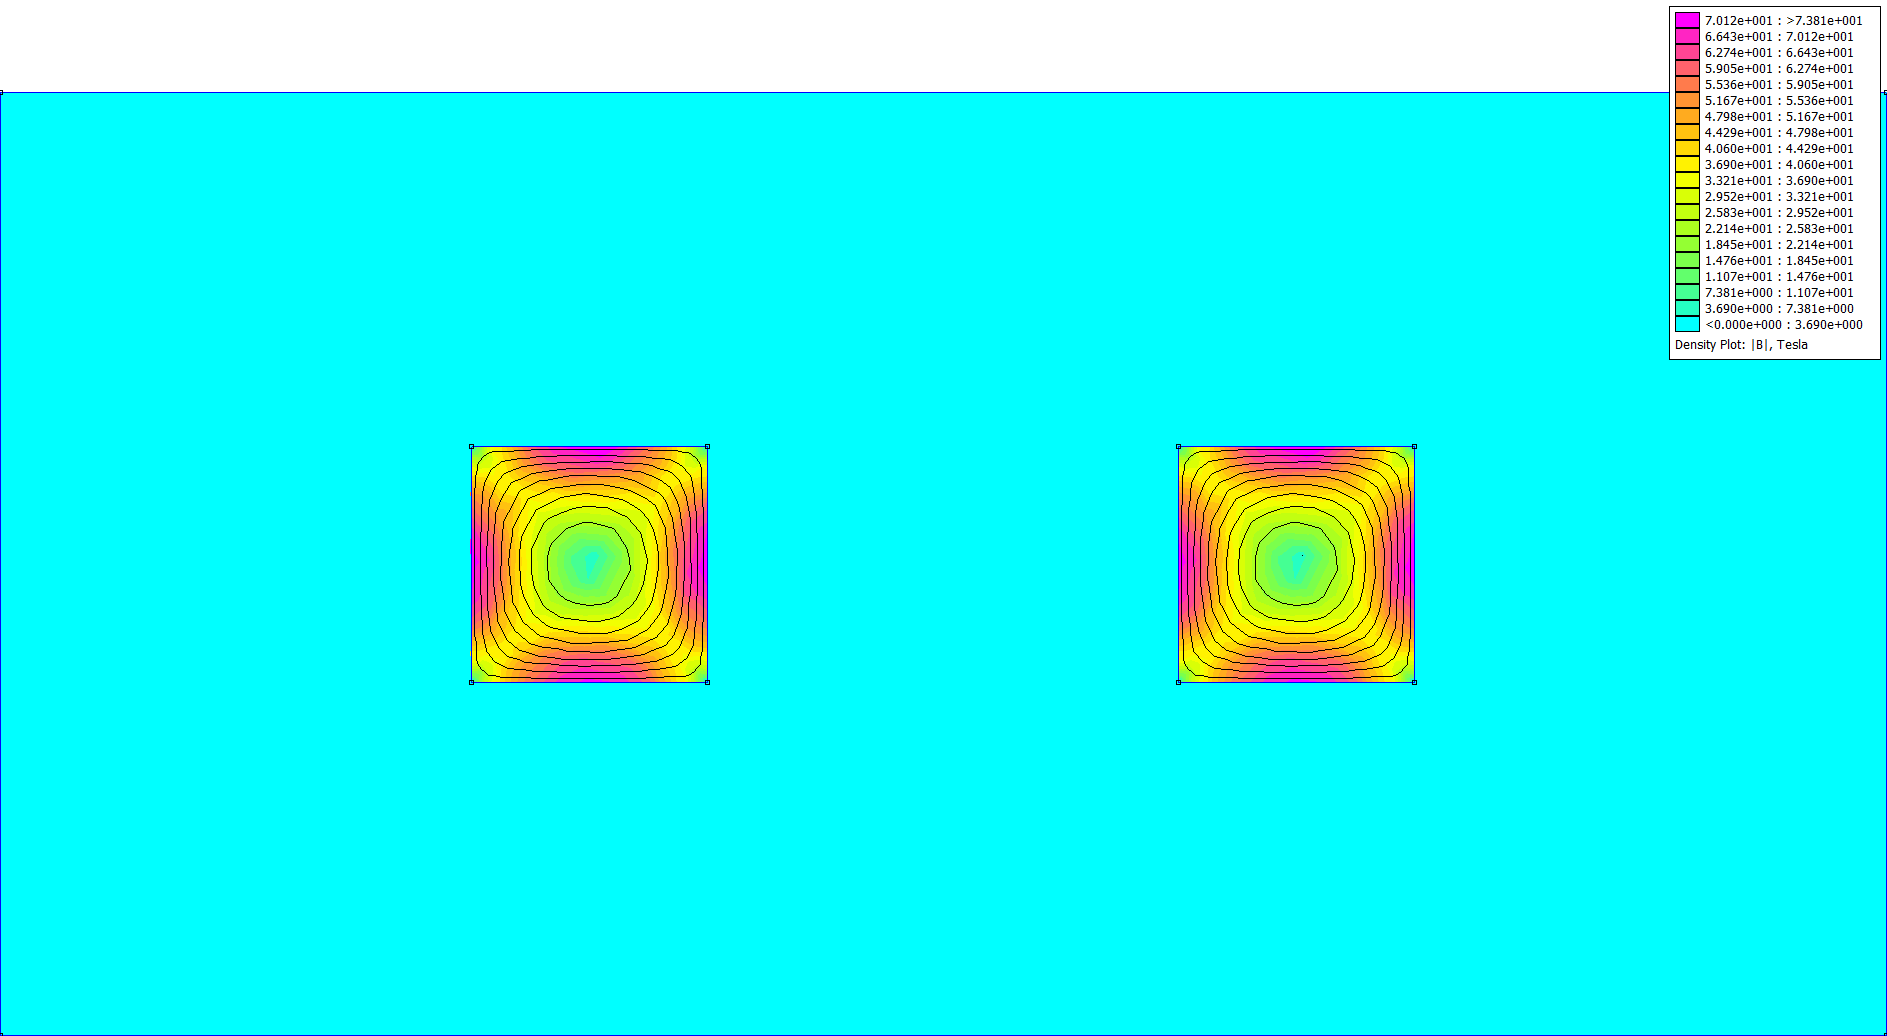
\includegraphics[width=.68\textwidth]{data/Stromfluss}
	\caption{Simulation des Stromflusses in FEMM}
	\label{fig:strom}
\end{figure}